\documentclass[border=10pt]{standalone}
\usepackage{tikz}
\begin{document}
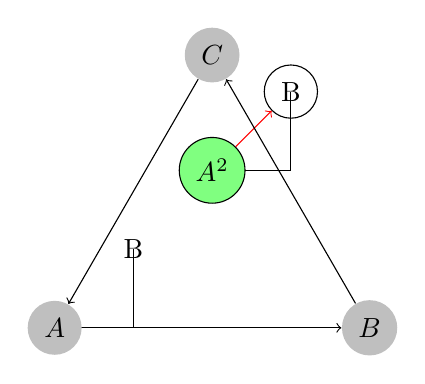
\begin{tikzpicture}
    \path[draw] (0, 0) -- (1, 0) -- (1, 1);
    \path[draw] (0, 0) node {A} -- (1, 0) -- (1, 1) node {B};
    \path[draw] (2, 2) node[draw, circle, fill=green!50] (nodeA) {$A^2$} -- (3, 2) -- (3, 3) node[draw, circle] (nodeB) {B};
    \path[draw, ->, red] (nodeA) -- (nodeB);

    \tikzstyle{every node} = [circle, fill=gray!50]
        \node (a) at (0, 0) {$A$};
        \node (b) at +(0: 4) {$B$};
        \node (c) at +(60: 4) {$C$};
        \foreach \from/\to in {a/b, b/c, c/a}
             \path[draw, ->] (\from) -- (\to);
\end{tikzpicture}
\end{document}